\chapter{Zalecenia dotyczące formatowania}
Większa część niniejszego rozdziału ma charakter informacyjny. Zamieszczone w nim informacje mają uzmysłowić czytelnikowi, jak wiele jest parametrów do ustawienia, by zredagowany dokument wyglądał ,,ładnie''. Parametry te poustawiano w szablonie. Wystarczy z niego skorzystać.

\section{Rozmiar i układ treści na stronach dokumentu}
Praca dyplomowa powinna być przygotowana do wydruku na papierze formatu A4 w orientacji pionowej.
Marginesy na stronach parzystych i nieparzystych powinny być jednakowe i mieć następujące wartości:
lewy = 25mm, prawy = 25mm, górny = 10mm, dolny = 15mm. Wielkość marginesów w szablonie sterowana jest parametrami przedstawionymi na rysunku~\ref{fig:pageLayout}. Margines dolny powinien być mierzony do linii bazowej tekstu stopki.
%\begin{figure}[htb]
%\centering
%\includegraphics[width=.7\linewidth]{rys03/pageLayout2}
%\caption{Kontrola marginesów i odstępów elementów na stronie} \label{fig:pageLayout}
%\end{figure}
\begin{figure}[htb]
	\setlayoutscale{0.43}
	\currentpage
	\drawparameterstrue
	%\drawpage
	\oddpagelayoutfalse
	\drawstock
	\caption{Układ strony nieparzystej dla dokumentu klasy \texttt{memoir}} \label{fig:pageLayout}
\end{figure}

Rzeczywisty układ strony zastosowany w niniejszym dokumencie przedstawiono na rysunku~\ref{fig:currentPageLayout}. Lewy i prawy margines są takie same, więc strony parzyste i nieparzyste wyglądają podobnie, z dokładnością do umiejscowienia notatek marginesowych. Taki rezultat zapewniło zastosowanie poniższych komend.
\begin{figure}[t]
	\setlayoutscale{0.43}
	\currentstock
	\oddpagelayouttrue
	\twocolumnlayoutfalse
	\drawmarginparstrue
	\drawparametersfalse
	\drawstock
	\caption{Rzeczywisty układ strony nieparzystej w tym dokumencie} \label{fig:currentPageLayout}
\end{figure}

\begin{lstlisting}[basicstyle=\footnotesize\ttfamily]
\setlength{\headsep}{10pt}
\setlength{\headheight}{13.6pt}
\setlength{\footskip}{\headsep+\headheight}
\setlength{\uppermargin}{\headheight+\headsep+1cm}
\setlength{\textheight}{\paperheight-\uppermargin-\footskip-1.5cm}
\setlength{\textwidth}{\paperwidth-5cm}
\setlength{\spinemargin}{2.5cm}
\setlength{\foremargin}{2.5cm}
\setlength{\marginparsep}{2mm}
\setlength{\marginparwidth}{2.3mm}
\checkandfixthelayout[fixed]
\linespread{1}
\setlength{\parindent}{14.5pt}
\end{lstlisting}


\section{Strona tytułowa}
Według ogólnouczelnianych zaleceń (tj.\ logotypu Politechniki Wrocławskiej) strona tytułowa powinna być zredagowana z~użyciem czcionki \texttt{garamond}. W oficjalnym wzorcu (patrz rysunek~\ref{fig:stronaTytulowa})
nie rozróżniono, czy dotyczy on pracy inżynierskiej czy magisterskiej.
\begin{figure}[b]
	\centering
	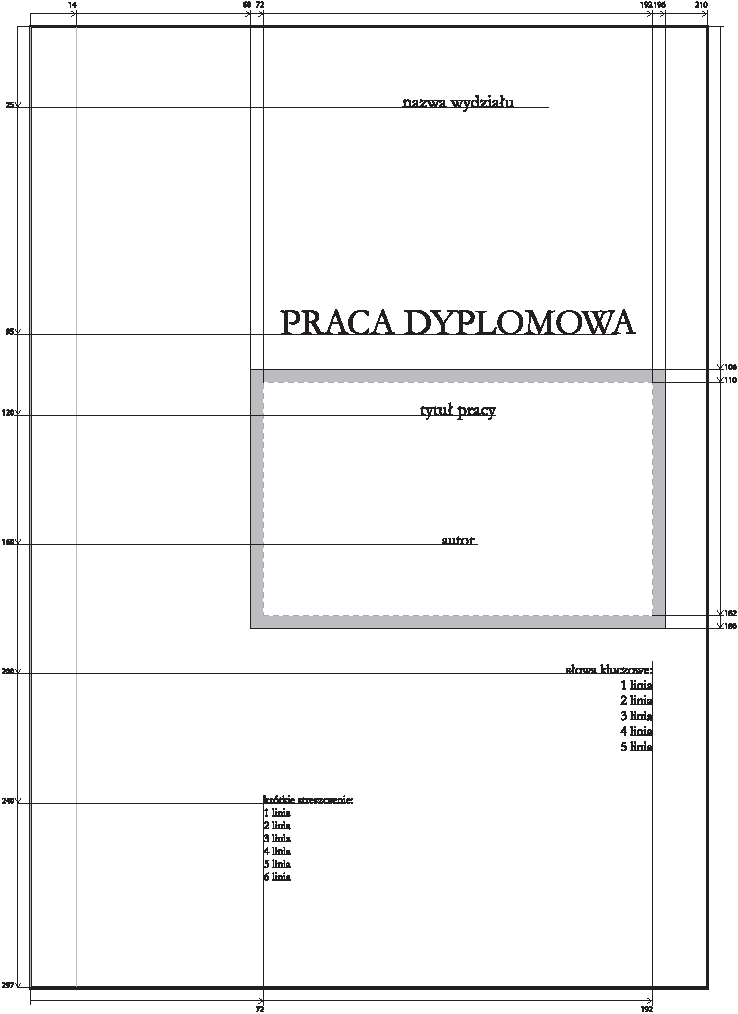
\includegraphics[width=.6\linewidth]{rys03/stronaTytulowa01}
	\caption{Oficjalny szablon strony tytułowej pracy dyplomowej, zamieszczony w dokumencie ,,System
		Identyfikacji Wizualnej Wrocław, sierpień 2016'' do pobrania ze strony \url{http://pwr.edu.pl/uczelnia/o-politechnice/materialy-promocyjne/logotyp} [dostęp dnia 07.12.2016]}
	\label{fig:stronaTytulowa}
\end{figure}
Nie uwzględniono również miejsca na nazwę specjalności ani kierunku oraz zapomniano o nazwisku promotora, jednostce, dacie i ocenie.  Za to określono  położenie słów kluczowych i~streszczenia. Ponieważ brakujące dane pojawiały się we wzorcach stron tytułowych stosowanych w~codziennej praktyce na Wydziałach, nie wiadomo do końca, czy oficjalny szablon należy stosować w 100 procentach. Dlatego w niniejszym dokumencie zastosowano własny wzorzec strony tytułowej (używany od lat) oraz podano wymagania odnośnie wzorca z~logotypu uczelnianego.

Ogólnouczelniane wymagania co do wielkości znaków na stronie tytułowej według uczelnianego logotypu są następujące:
\begin{lstlisting}[basicstyle=\footnotesize\ttfamily]
Nazwa jednostki organizacyjnej: Garamond 16 pt
Napis "PRACA DYPLOMOWA INŻYNIERSKA": Garamond 32 pt
Tytuł pracy: Garamond 16 pt
Autor: Garamond 14 pt
Słowa kluczowe: Garamond 12 pt
Krótkie streszczenie: Garamond 10 pt
\end{lstlisting}

W grudniu 2021 na stronie Wydziału Informatyki i Teleinformatyki pojawił się nowy szablon pracy dyplomowej z nowym wyglądem strony tytułowej. Nie zgadza się on z szablonem ogólnouczelnianym. Co więcej, w szablonie tym nie uwzględnia się już geometrii ,,okienka'' na tytuł, inaczej nazwano promotora (teraz jest to ,,Opiekun pracy''), inaczej zadeklarowane są wielkości czcionek oraz stosowane wielkości znaków (zrezygnowano w kilku miejscach ze stosowania kapitalików).

W niniejszym szablonie starano się odzwierciedlić układ strony tytułowej przedstawiony na stronie Wydziału. I tak wymagania co do wielkości znaków na stronie tytułowej według wzorca użytego w niniejszym dokumencie są następujące
\begin{lstlisting}[basicstyle=\footnotesize\ttfamily]
Politechnika Wrocławska (Garamond Bold 20pt 22pt)
Wydział Informatyki i Teleinformatyki (Garamond Bold 16pt 18pt)
Kierunek: Jakiś kierunek (Garamond 14pt 16pt, Garamond Bold 14pt 16pt)
Specjalność: Jakaś specjalność (Garamond 14pt 16pt, Garamond Bold 14pt 16pt)
{P}RACA {D}YPLOMOWA (Garamond 26pt 28pt, Garamond 24pt 26pt)
{I}NŻYNIERSKA (Garamond 26pt 28pt, Garamond 24pt 26pt)
Tytuł pracy w języku polskim (Garamond Bold 18pt 20pt)
Title in English (Garamond Bold 18pt 20pt)
% AUTOR: (Garamond 16pt 18pt) - zamarkowane
Imię Nazwisko (Garamond Bold 16pt 18pt)
Opiekun pracy (Garamond 14pt 16pt)
tytuł/stopień naukowy, Imię Nazwisko (Garamond 14pt 16pt)
%OCENA PRACY: (Garamond 16pt 18pt) - zamarkowane
WROCŁAW, 2021 (Garamond 14pt 16pt)
\end{lstlisting}

W szablonie zastosowano pakiet \texttt{ebgaramond}. Dostarcza on klonu czcionki \texttt{garamond}, jednak bez kształtu \texttt{slanted} i z pewnymi brakami. Na przykład zamiast literki ,,ł'' w zbiorze \texttt{EBGaramond08 Italic} renderuje się samo ,,l'' (braku tego nie ma zbiór \texttt{EBGaramond12}).  Zaletą pakietu  w porównaniu do innych jest to, że generalnie dobrze obsługiwane są w nim polskie znaki oraz że pakiet ten można znaleźć w różnych dystrybucjach latexa (\texttt{MikTeX} instaluje go automatycznie).

\section{Krój i wielkość czcionek}
Główny tekst pracy powinien być zredagowany z wykorzystaniem czcionki \texttt{Times}, typ normalny, o wysokości 12pt, z odstępem między liniami równym 14.5pt. Istnieje możliwość zmiany odstępu między liniami za pomocą komendy \verb?\linespread?, jednak zaleca się pozostawienie tego odstępu jak w niniejszym dokumencie (\verb?\linespread{1}?). Wymagania odnośnie kroju pisma pozostałych elementów (nagłówków, stopek itp.) zamieszczono w tabeli~\ref{tab:secfonts}.

W szablonie zastosowano czcionkę \texttt{texgyre-termes} (dostarcza ją pakiet \texttt{tgtermes}). Czcionka ta jest klonem czcionki \texttt{Times}, w którym obsługiwane jest środkowoeuropejskie kodowanie znaków (podobnie jak w przypadku czcionki \texttt{ebgaramond}, dzięki czemu polskie literki nie są zlepkami dwóch znaków lecz pojedynczymi znakami).

Wszelkie przykłady źródeł kodu (fragmenty programów, komendy linii poleceń), nazwy plików i uruchamianych programów powinny być pisane czcionką maszynową. W szablonie czcionką maszynową jest \texttt{t1xtt}. Czcionka ta obsługuje polskie znaki. Dostarcza ją pakiet \texttt{txfonts}, który należy wcześniej zainstalować (MiKTeX zainstaluje go automatycznie podczas pierwszej kompilacji szablonu).

% https://en.wikibooks.org/wiki/LaTeX/Lengths
% there are two different point sizes.  A pdf point is 1/72 inch.  A LaTeX point is 1/72.27 inch.  Thus,
% the LaTeX point is slightly smaller than a pdf point.

%\texttt{baselineskip}: \printlength{\baselineskip}\\
%\texttt{beforesecskip}: \printlength{\beforesecskip}\\
%\texttt{aftersecskip}: \printlength{\aftersecskip}\\
%\texttt{topskip}: \printlength{\topskip}\\
%\texttt{fontsize}: \showFontSize\\

\begin{table}[htb]
	\centering
	\caption{Zestawienie czcionek elementów podziału dokumentu, tekstu wiodącego, nagłówka i stopki oraz podpisów (Rozm. -- rozmiar czcionki, Odst. -- \texttt{baselineskip})}
	\label{tab:secfonts}\small
	\begin{tabularx}{\linewidth}{|ll@{\hskip 5pt}l@{\hskip 5pt}lX|} \hline
		Element              & Przykład                                   & Czcionka                    & Rozm.  & Odst.  \\ \hline\hline
		Nr rozdziału         & {\huge\bfseries Rozdział 1 }               & \verb?\huge\bfseries?       & 25pt   & 30pt   \\
		Tytuł rozdziału      & {\Huge\bfseries Wstęp }                    & \verb?\Huge\bfseries?       & 30pt   & 37pt   \\
		Nr i tytuł sekcji    & {\Large\bfseries 1.1. Wprowadzenie }       & \verb?\Large\bfseries?      & 17pt   & 22pt   \\
		Nr i tytuł podsekcji & {\large\bfseries 1.1.1. Cel szczegółowy }  & \verb?\large\bfseries?      & 14.5pt & 18pt   \\
		Tytuł podpodsekcji   & {\normalsize\bfseries Założenia }          & \verb?\normalsize\bfseries? & 12pt   & 14.5pt \\
		Tytuł paragrafu      & {\normalsize\bfseries  Podstawy } Opis ... & \verb?\normalsize\bfseries? & 12pt   & 14.5pt \\
		Tekst wiodący        & {\normalsize Niniejszy dokument ... }      & \verb?\normalsize?          & 12pt   & 14.5pt \\
		Nagłówek strony      & {\small\itshape 3.2. Czcionka wiodąca ...} & \verb?\small\itshape?       & 11pt   & 13.6pt \\
		Stopka strony        & {\small Imię Nazwisko: ...}                & \verb?\small?               & 11pt   & 13.6pt \\
		Podpisy tabel        & {\small Tab.~3.1: Zestawienie ...}         & \verb?\small?               & 11pt   & 13.6pt \\
		Podpisy rysunków     & {\small Rys.~3.1: Oficjalny ...}           & \verb?\small?               & 11pt   & 13.6pt \\\hline
	\end{tabularx}
\end{table}
%\texttt{fontsize}: \showFontSize

Jeśli w pracy zostaną użyte otoczenia matematyczne, to w dokumencie wynikowym pojawią się dodatkowe czcionki (domyślne latexowe czcionki do wyrażeń matematycznych). Dzięki zastosowaniu opcji \texttt{extrafontsizes} w klasie \texttt{memoir} nie dość, że otrzymuje się większe czcionki (30pt), to jeszcze zamiast \texttt{Computer Modern} do wzorów matematycznych jest stosowana czcionka \texttt{Latin Modern} (wywodząca się z \texttt{Computer Modern}).
Stąd lista wszystkich użytych czcionek może być następująca:
\begin{lstlisting}[basicstyle=\footnotesize\ttfamily]
EBGaramond12-Regular
GaramondNo8-Reg-Norml
TeXGyreTermes-Regular-Normalna
TeXGyreTermes-Bold-Pogrubiona
TeXGyreTermes-Italic-Normalna
t1xtt-Nomal
LMMathItalic12-Regular
LMMathSymbols10-Regular
LMMathExtension10-Regular
LMRoman8-Regular
\end{lstlisting}

Aby wykorzystać te czcionki poza systemem LaTeX, wystarczy pobrać je spod adresów (ważnych na dzień
1.04.2016):
\url{https://www.ctan.org/tex-archive/fonts/cm/ps-type1/bakoma/ttf/?lang=en}, \url{http://www.gust.org.pl/projects/e-foundry/latin-modern}, \url{http://www.gust.org.pl/projects/e-foundry/tex-gyre}, \url{https://bitbucket.org/georgd/eb-garamond/downloads},
a następnie zainstalować w systemie. Dzięki temu można będzie np.~edytować rysunki używając dokładnie tej samej czcionki, co czcionka użyta w dokumencie.

\section{Formatowanie bloków tekstu}
Każdy rozdział pracy powinien rozpoczynać się od nowej strony. Jej wygląd powinien być kontrolowany parametrami pokazanymi na rysunku~\ref{fig:LayChap}.
\begin{figure}[t]
	\setlayoutscale{0.6}
	\centering
	\chapterdiagram
	\caption{Parametry sterujące wielkościami odstępów na stronie z tytułem rozdziału}
	\label{fig:LayChap}
\end{figure}
W niniejszym szablonie (dokument klasy \texttt{memoir} z opcją \texttt{[12pt]}) przyjęto następujące wartości tych parametrów:
\begin{itemize}
	\item \verb?\beforechapskip? (\printlength{\beforechapskip}) + \verb?\baselineskip? of \verb+\huge+ (30pt) + \verb+\topskip+ (\printlength{\topskip}) = 92pt (3.246cm)
	\item \verb?\midchapskip? (\printlength{\midchapskip}) + \verb?\baselineskip? of \verb+\Huge+ (37pt) = 57 pt (2.011cm)
	\item \verb?\afterchapskip? (\printlength{\afterchapskip}) + \verb+\baselineskip+ of \verb+\normalsize+ (14.5pt) = 54.5pt (1.923cm)
\end{itemize}

Nieco kłopotów może sprawić dobre ustawienie na stronie tytułów nienumerowanych rozdziałów oraz list generowanych automatycznie (Skróty, Spis treści, Spis rysunków, Spis tabel, Indeks rzeczowy). W szablonie w tym celu zdefiniowano nowy styl rozdziału komendami jak niżej (w szablonie są to komendy zamarkowane)
\begin{lstlisting}[basicstyle=\footnotesize\ttfamily]
\newlength{\linespace}
\setlength{\linespace}{-\beforechapskip-\topskip+\headheight+\topsep}
\makechapterstyle{noNumbered}{%
\renewcommand\chapterheadstart{\vspace*{\linespace}}
}
\end{lstlisting}
oraz dokonano przełączenia stylów rozdziałów komendami \verb?\chapterstyle{nonumbered}? oraz \verb?\chapterstyle{default}? podczas dołączania do dokumentu wymienionych nienumerowanych rozdziałów i list. Aby ,,podnieść do góry'' tytuły nienumerowanych rozdziałów (gdy jest to rzeczywiście konieczne) wystarczy odmarkować wspomniane komendy.

Tytuły rozdziałów, sekcji, podsekcji itd.\ nie powinny kończyć się kropką. Odległości pomiędzy tekstem wiodącym a tytułem sekcji powinien być regulowany parametrami pokazanymi na rysunku~\ref{fig:LaySec}.
\begin{figure}[t]
	%\setlayoutscale{1}
	\runinheadfalse
	\drawparameterstrue
	\drawheading{\Large\bfseries}
	\caption{Kontrola ustawień odległości w tytułach kolejnych sekcji}
	\label{fig:LaySec}
\end{figure}
Rozmiar \verb?\baselineskip? zależy od rozmiaru czcionki (zobacz tabela~\ref{tab:secfonts}), zaś \texttt{beforeskip} i \texttt{secskip} od poziomu sekcji. W niniejszym szablonie przyjęto następujące wartości tych parametrów (są to wartości dobierane elastycznie podczas kompilacji):
\begin{itemize}
	\item \texttt{indent = 14.5pt}
	\item \texttt{parskip = \printlength{\parskip}}
	\item \texttt{beforesecskip = \printlength{\beforesecskip}}
	\item \texttt{aftersecskip = \printlength{\aftersecskip}}
	\item \texttt{beforesubsecskip = \printlength{\beforesubsecskip}}
	\item \texttt{aftersubsecskip = \printlength{\aftersubsecskip}}
	\item \texttt{beforesubsubsecskip = \printlength{\beforesubsecskip}}
	\item \texttt{aftersubsubsecskip = \printlength{\aftersubsecskip}}
\end{itemize}

W szablonie obowiązują również następujące wartości parametrów odpowiedzialnych za odstępy pomiędzy pływającymi figurami, tekstami oraz tekstem i figurą:
\begin{itemize}
	\item \texttt{floatsep = \printlength{\floatsep}}
	\item \texttt{intextsep = \printlength{\intextsep}}
	\item \texttt{textfloatsep = \printlength{\textfloatsep}}
\end{itemize}

Pierwsza linia pierwszego akapitu w bloku (po tytule rozdziału, sekcji, podsekcji, podpodsekcji) nie może mieć wcięcia. Pierwsze linie w kolejnych akapitach już powinny mieć wcięcie równe \texttt{14.5pt}. Tekst w akapitach powinien być wyrównany z obu stron.


Strony powinny być numerowane numeracją ciągłą (sekwencja arabskich cyfr). Numery stron powinny być umieszczone w ich stopkach (tj.\ tak jak w niniejszym dokumencie). Wyjątkiem są tutaj pierwsze strony rozdziałów oraz strona tytułowa -- na nich numery nie powinny się pojawić.

\section{Opisy tabel i rysunków}
Podpisy powinny być umieszczane pod rysunkami lub nad tabelami wraz z etykietą składającą się ze skrótu Rys.\ lub Tab.\ oraz numeru. Podpisy te nie powinny mieć końcowej kropki. Numery występujący w podpisach powinny zaczynać się numerem rozdziału, po którym następuje kolejny numer rysunku lub tabeli w obrębie rozdziału. Etykieta powinna kończyć się dwukropkiem, po którym następuje tekst podpisu. Numer rozdziału powinien być rozdzielony kropką od kolejnego numeru w rysunku bądź tabeli w rozdziale (liczniki tabel i rysunków są rozłączne). Należy pamiętać o tym, żeby w całej pracy tabele miały podobny wygląd (rodzaj czcionki, ewentualne pogrubienia w nagłówku itp.). %Źródła należy podawać pod tabelą.

\section{Przypisy dolne}
Istnieje możliwość zamieszczania przypisów na dole strony, choć nie jest to zalecane (przykładowo~\footnote{Tekst przypisu}). Sposób parametryzowania ich wyglądu pokazano na rysunku~\ref{fig:fp}. W szablonie wykorzystano następujące, domyślne wartości tych parametrów:
\begin{lstlisting}[basicstyle=\footnotesize\ttfamily]
\footins = 12pt \footnotesep = 8pt
\baselineskip = 10pt note separation = 40pt
rule thickness = 0.4pt
rule length = 0.25 times the \textwidth
\end{lstlisting}
\begin{figure}[htb]
	\setlayoutscale{0.3}
	\drawfootnote
	\caption{Parametry sterujące przypisami dolnymi} \label{fig:fp}
\end{figure}
%\tryfootins
%\tryfootnotesep
%\tryfootnotebaseline
%\tryfootruleheight
%\tryfootrulefrac

%\footins = 12pt \footnotesep = 8pt
%\baselineskip = 10pt note separation = 40pt
%rule thickness = 0.4pt
%rule length = 0.25 times the \textwidth

\section{Formatowanie spisu treści}
W klasie memoir istnieją komendy pozwalające dość dobrze zarządzać wyglądem spisu treści. Na rysunku~\ref{fig:ltoc} pokazano, za pomocą jakich parametrów można wpływać na finalną jego postać. W szablonie wykorzystano następujące, domyślne ich wartości:
\begin{lstlisting}[basicstyle=\footnotesize\ttfamily]
indent = 18pt
numwidth = 28pt
\@tocrmarg = 31pt
\@pnumwidth = 19pt
\@dotsep = 4.5
\end{lstlisting}

\begin{figure}[h]
	\setlayoutscale{0.5}
	\drawtoc
	\caption{Parametryzacja wyglądu spisu treści} \label{fig:ltoc}
\end{figure}

%\begin{figure}
%\setlayoutscale{0.8}
%\currenttoc
%\drawparametersfalse
%\drawtoc
%\caption{Parametry definiujące postać spisu treści w niniejszym szablonie} \label{fig:thistoc}
%\end{figure}

\section{Formatowanie list wyliczeniowych i wypunktowań}
Standardowo sposób formatowania list można parametryzować jak pokazano na rysunku~\ref{fig:listlay}. Jednak czasem trudno poradzić sobie z niektórymi rzeczami, jak np.~znakami wypunktowania. Dlatego w szablonie wykorzystano pakiet \texttt{enumi}. Pozwala on na łatwe zarządzanie wyglądem list. W szablonie zastosowano następujące globalne ustawienia dla tego pakietu:
\begin{lstlisting}[basicstyle=\footnotesize\ttfamily]
\usepackage{enumitem}
\setlist{noitemsep,topsep=4pt,parsep=0pt,partopsep=4pt,leftmargin=*}
\setenumerate{labelindent=0pt,itemindent=0pt,leftmargin=!,label=\arabic*.}
\setlistdepth{4}
\setlist[itemize,1]{label=$\bullet$}
\setlist[itemize,2]{label=\normalfont\bfseries\textendash}
\setlist[itemize,3]{label=$\ast$}
\setlist[itemize,4]{label=$\cdot$}
\renewlist{itemize}{itemize}{4}
\end{lstlisting}
\begin{figure}[h]
	\centering
	\setlayoutscale{0.4}
	\drawparameterstrue
	\drawlist
	\caption{Parametryzacja list wyliczeniowych i wypunktowań}\label{fig:listlay}
\end{figure}

W~podrozdziale~\ref{sec:Styl} pokazano przykład wykorzystania możliwości komend oferowanych w~pakiecie \texttt{enumi}.

\section{Wzory matematyczne}
Wzory matematyczne, jeśli mają być osobnymi formułami, powinny być wycentrowane, z~numeracją umieszczoną na końcu linii i ujętą w okrągłe nawiasy (zobacz równanie (\ref{eq:xdx})). Numery równań powinny zawierać numer rozdziału oraz kolejny numer równania w obrębie rozdziału (podobnie jak przy numerowaniu rysunków i tabel). Spełnienie tych warunków zapewnia otoczenie \verb?equation?. Nie wszystkie formuły trzeba numerować (nienumerowane wzory można osiągnąć stosując otoczenie \verb?\equation*?). Właściwie należy numerować tylko te, do których tworzy się jakieś odniesienia w tekście. Jeśli wzory umieszczane są w linijce tekstu, to można zastosować otoczenie matematyczne inline, jak w~przykładzie $\int_{0}^{10\nu\sum i}{x dx}$ (wyprodukowanym komendą \verb?$\int_{0}^{10\nu\sum i}{x dx}$?). Tylko że wtedy może dojść do rozszerzenia odstępów pomiędzy liniami tekstu (aby zmieścił się wzór).
\begin{equation}\label{eq:xdx}
	\int_{0}^{10\nu\sum i}{x dx}
\end{equation}
